\documentclass{article}
\usepackage[top=0.1in, bottom=0.5in, left=0.5in, right=0.5in]{geometry}
% \usepackage[utf8]{inputenc}
\usepackage[utf8]{inputenc}
\usepackage{amsmath}
\usepackage{graphicx}
\begin{document}
\section{Introduction}
We began our journey with word vectors. We looked at vectors on 2D plane in using python to understand analogies and importance of word vectors. Then we moved to RNNS (Recurrent Neural Networks). This architecture had vanishing gradients problem (gradients diminish exponentially as they are propagated back through time) which prevented it from learning long-term dependences in sequences. This issue was partially resolved by LSTMS (Long Short-Term Memory). We used LSTMs for neural machine translation. This was an interesting task. However, it was slow due to its sequential processing of input embeddings. We then moved to transformers to utilize the parallel processing capabilities of GPUs.
\subsection{Recurrent Neural Networks(RNNs)}
Let's first talk a briefly about RNNs. RNNs are a class of Neural Networks which take inputs sequentially and produce a hidden state.


\begin{figure}[ht!]
\centering
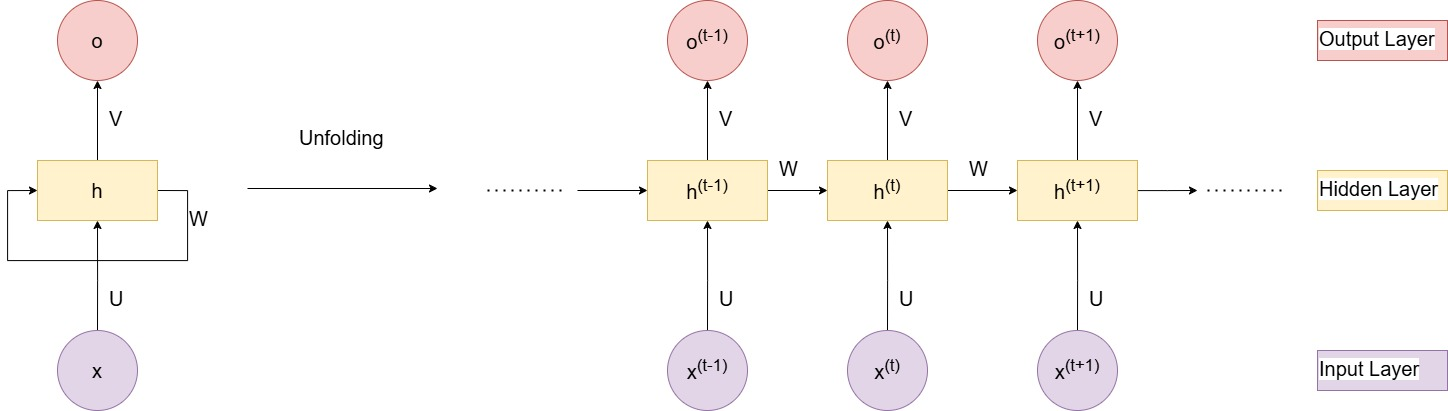
\includegraphics[width=90mm]{Images/RNN.jpg}
\caption{Basic RNN structure. Here x is input sequence, o is output sequence, and h is the hidden state. U, V, and W are training weights\label{overflow}}
\end{figure}

The hidden state is calculated using the following equation:
\begin{equation} \label{eqn}
h_t = {g(Uh_{t-1}+Wx_{t-1})}
\end{equation}
Here, \(h_t\) is the hidden state at time t, g is the activation function.

Then, using the following equation output is calculated:
\begin{equation} \label{eqn}
o_t = {f(Vh_t)}
\end{equation}
Here, \(o_t\) is the output at time t, f is another activation function.

We studied bidirectional RNNs. \textbf{Biderection RNN} combines two independent RNNs, one where the input is processed from the start to the end and the other where the input is processed from the end to the start. We then concatenate the two hidden states into one vector. This vector captures both left and right contexts of an input at each point in time. Vector concatenation is shown like this:
\begin{equation} \label{eqn}
h_t={[h_t^f;h_t^b]}
\end{equation}
RNNs are good at learning short term dependencies but fail to learn short term dependencies becauuse of the vanishing graddients problem.
\section{Tasks}
\subsection{Week 1}
\subsection{Rooshan Khan: Attention Method in bert.py}
In this method we had to implement Attention method from class BertSelfAttention. The attention mechanism is given by:
\begin{equation} \label{eqn}
Attention(Q,K,V) = {softmax(\frac{QK^T}{\sqrt{d_k}})V}
\end{equation}
where \( Q \), \( K \), and \( V \) represent the query, key, and value matrices, respectively, and \( d_k \) is the dimension of the key vectors.

I used method \( torch.matmul \) to multiply \( Q \) and transpose of \( K \). I multiplied the result with \( attention\_mask \) to apply the mask. The dimensions of attention\_mask are \( [bs, 1, 1, seq\_len] \). The attention mask distinguishes between non-padding tokens and padding tokens. The non-padding tokens have a value of 0 while padding tokens have a value of a large negative number. The dimensions of key\_layer,query\_layer and value\_layer are \( [bs, num\_attention\_heads, seq\_len, attention\_head\_size] \)

Now I will tell how I concatenated all heads. When we transpose the tensor we change the shape of the tensor from \( [bs,num\_attention\_heads,seq\_len,attention\_head\_size] \) to \( [bs,seq\_len,num\_attention\_heads,attention\_head\_size] \). This enables us to reshape the tensor to \( [bs,seq\_len,num\_attention\_heads*attention\_head\_size] \). After applying the transpose method the data sequence does not follow a contiguous order so we need to use \textbf{contiguous} method before using the \textbf{view}\ method.

\subsection{Hussnain Amjad: add\_norm Method in bert.py}
The add\_norm function is a critical component of the Transformer architecture, ensuring stable and effective training by combining residual connections, dropout, and layer normalization. It transforms the output of a sub-layer using a dense layer, applies dropout for regularization, and then adds it to the sub-layer's input through a residual connection. This output is further normalized using a layer norm to maintain consistent feature scaling across the model. This combination not only stabilizes gradient flow but also mitigates issues like vanishing gradients and overfitting, enabling the model to learn deeper representations effectively.

\subsection{Areesha Noor: forward Method in bert.py}
In the Bertlayer class, we have a forward function following add-norm function. The forward function is responsible for the overall flow from multi-head attention, followed by add-norm, a  feed-forward layer and then another add-norm operation in the BERT architecture.So, the forward function transforms the input (hidden states) through series of sequential operations which represents the contextual relationships between tokens of sentences.

This was implemented by first computing attention scores by using "forward function" in  BertSelfAttention class. By using this class, the hidden_states are processed through attention mechanism. The output of the attention is of the same size as of input \(i.e R^(NxD) \). Then, add-norm operation is applied to the attention scores using add\_norm function in BertLayer class. Here, the residual connection is applied to attention layer. Next, for implementation of feed-forward layer, the normalized output of attention layer (attention\_out\_norm) is first passed through dense linear transformation (interm\_dense). Mathematically, 

\begin{equation} \label{eqn}
feedforward_out=W_1⋅attention_out_norm+b_1
\end{equation}

where 
W1= weight matrix 
b1 = bias vector 

Then, activation function GELU (Gaussian Error Linear Unit) is applied to introduce non-linearity in the model. Mathematically,
GELU = 0.5⋅x(1+tanh(2/π)⋅(x+0.044715x^3)))
 Finally, add-norm is applied by passing the feed-forward network through add-norm function for residual connection.
\end{document}